% Generated by Sphinx.
\def\sphinxdocclass{report}
\documentclass[a4paper,10pt,english]{sphinxmanual}
\usepackage[utf8]{inputenc}
\DeclareUnicodeCharacter{00A0}{\nobreakspace}
\usepackage{cmap}
\usepackage[T1]{fontenc}
\usepackage{babel}
\usepackage{mathpazo}
\usepackage[Sonny]{fncychap}
\usepackage{longtable}
\usepackage{sphinx}
\usepackage{multirow}

\addto\captionsenglish{\renewcommand{\figurename}{Fig. }}
\addto\captionsenglish{\renewcommand{\tablename}{Table }}
\floatname{literal-block}{Listing }

\usepackage{ManualStyle}

\title{Manuale operativo MongoDB}
\date{March 01, 2016}
\release{0.1}
\author{AXANT}
\newcommand{\sphinxlogo}{}
\renewcommand{\releasename}{Release}
\makeindex

\makeatletter
\def\PYG@reset{\let\PYG@it=\relax \let\PYG@bf=\relax%
    \let\PYG@ul=\relax \let\PYG@tc=\relax%
    \let\PYG@bc=\relax \let\PYG@ff=\relax}
\def\PYG@tok#1{\csname PYG@tok@#1\endcsname}
\def\PYG@toks#1+{\ifx\relax#1\empty\else%
    \PYG@tok{#1}\expandafter\PYG@toks\fi}
\def\PYG@do#1{\PYG@bc{\PYG@tc{\PYG@ul{%
    \PYG@it{\PYG@bf{\PYG@ff{#1}}}}}}}
\def\PYG#1#2{\PYG@reset\PYG@toks#1+\relax+\PYG@do{#2}}

\expandafter\def\csname PYG@tok@gu\endcsname{\let\PYG@bf=\textbf\def\PYG@tc##1{\textcolor[rgb]{0.50,0.00,0.50}{##1}}}
\expandafter\def\csname PYG@tok@gt\endcsname{\let\PYG@bf=\textbf\def\PYG@tc##1{\textcolor[rgb]{0.64,0.00,0.00}{##1}}}
\expandafter\def\csname PYG@tok@gs\endcsname{\let\PYG@bf=\textbf\def\PYG@tc##1{\textcolor[rgb]{0.00,0.00,0.00}{##1}}}
\expandafter\def\csname PYG@tok@gr\endcsname{\def\PYG@tc##1{\textcolor[rgb]{0.94,0.16,0.16}{##1}}}
\expandafter\def\csname PYG@tok@cm\endcsname{\let\PYG@it=\textit\def\PYG@tc##1{\textcolor[rgb]{0.40,0.39,0.52}{##1}}}
\expandafter\def\csname PYG@tok@gp\endcsname{\def\PYG@tc##1{\textcolor[rgb]{0.45,0.33,0.20}{##1}}}
\expandafter\def\csname PYG@tok@m\endcsname{\def\PYG@tc##1{\textcolor[rgb]{0.60,0.00,0.00}{##1}}}
\expandafter\def\csname PYG@tok@na\endcsname{\def\PYG@tc##1{\textcolor[rgb]{0.77,0.63,0.00}{##1}}}
\expandafter\def\csname PYG@tok@go\endcsname{\def\PYG@tc##1{\textcolor[rgb]{0.53,0.53,0.53}{##1}}}
\expandafter\def\csname PYG@tok@ge\endcsname{\let\PYG@it=\textit\def\PYG@tc##1{\textcolor[rgb]{0.00,0.00,0.00}{##1}}}
\expandafter\def\csname PYG@tok@gd\endcsname{\def\PYG@tc##1{\textcolor[rgb]{0.64,0.00,0.00}{##1}}}
\expandafter\def\csname PYG@tok@il\endcsname{\def\PYG@tc##1{\textcolor[rgb]{0.60,0.00,0.00}{##1}}}
\expandafter\def\csname PYG@tok@cs\endcsname{\let\PYG@it=\textit\def\PYG@tc##1{\textcolor[rgb]{0.40,0.39,0.52}{##1}}}
\expandafter\def\csname PYG@tok@cp\endcsname{\def\PYG@tc##1{\textcolor[rgb]{0.40,0.39,0.52}{##1}}}
\expandafter\def\csname PYG@tok@gi\endcsname{\def\PYG@tc##1{\textcolor[rgb]{0.00,0.63,0.00}{##1}}}
\expandafter\def\csname PYG@tok@gh\endcsname{\let\PYG@bf=\textbf\def\PYG@tc##1{\textcolor[rgb]{0.00,0.00,0.50}{##1}}}
\expandafter\def\csname PYG@tok@ni\endcsname{\def\PYG@tc##1{\textcolor[rgb]{0.81,0.36,0.00}{##1}}}
\expandafter\def\csname PYG@tok@ld\endcsname{\def\PYG@tc##1{\textcolor[rgb]{0.00,0.00,0.00}{##1}}}
\expandafter\def\csname PYG@tok@nl\endcsname{\def\PYG@tc##1{\textcolor[rgb]{0.96,0.47,0.00}{##1}}}
\expandafter\def\csname PYG@tok@nn\endcsname{\def\PYG@tc##1{\textcolor[rgb]{0.00,0.00,0.00}{##1}}}
\expandafter\def\csname PYG@tok@no\endcsname{\def\PYG@tc##1{\textcolor[rgb]{0.00,0.00,0.00}{##1}}}
\expandafter\def\csname PYG@tok@s2\endcsname{\def\PYG@tc##1{\textcolor[rgb]{0.45,0.09,0.11}{##1}}}
\expandafter\def\csname PYG@tok@nb\endcsname{\def\PYG@tc##1{\textcolor[rgb]{0.00,0.00,0.00}{##1}}}
\expandafter\def\csname PYG@tok@nc\endcsname{\def\PYG@tc##1{\textcolor[rgb]{0.86,0.40,0.00}{##1}}}
\expandafter\def\csname PYG@tok@nd\endcsname{\def\PYG@tc##1{\textcolor[rgb]{0.53,0.53,0.53}{##1}}}
\expandafter\def\csname PYG@tok@ne\endcsname{\let\PYG@bf=\textbf\def\PYG@tc##1{\textcolor[rgb]{0.80,0.00,0.00}{##1}}}
\expandafter\def\csname PYG@tok@nf\endcsname{\def\PYG@tc##1{\textcolor[rgb]{0.86,0.40,0.00}{##1}}}
\expandafter\def\csname PYG@tok@nx\endcsname{\def\PYG@tc##1{\textcolor[rgb]{0.00,0.00,0.00}{##1}}}
\expandafter\def\csname PYG@tok@si\endcsname{\def\PYG@tc##1{\textcolor[rgb]{0.45,0.09,0.11}{##1}}}
\expandafter\def\csname PYG@tok@sh\endcsname{\def\PYG@tc##1{\textcolor[rgb]{0.45,0.09,0.11}{##1}}}
\expandafter\def\csname PYG@tok@vi\endcsname{\def\PYG@tc##1{\textcolor[rgb]{0.00,0.00,0.00}{##1}}}
\expandafter\def\csname PYG@tok@py\endcsname{\def\PYG@tc##1{\textcolor[rgb]{0.00,0.00,0.00}{##1}}}
\expandafter\def\csname PYG@tok@nt\endcsname{\let\PYG@bf=\textbf\def\PYG@tc##1{\textcolor[rgb]{0.00,0.27,0.38}{##1}}}
\expandafter\def\csname PYG@tok@nv\endcsname{\def\PYG@tc##1{\textcolor[rgb]{0.00,0.00,0.00}{##1}}}
\expandafter\def\csname PYG@tok@s1\endcsname{\def\PYG@tc##1{\textcolor[rgb]{0.45,0.09,0.11}{##1}}}
\expandafter\def\csname PYG@tok@vg\endcsname{\def\PYG@tc##1{\textcolor[rgb]{0.00,0.00,0.00}{##1}}}
\expandafter\def\csname PYG@tok@kd\endcsname{\let\PYG@bf=\textbf\def\PYG@tc##1{\textcolor[rgb]{0.00,0.00,0.00}{##1}}}
\expandafter\def\csname PYG@tok@vc\endcsname{\def\PYG@tc##1{\textcolor[rgb]{0.00,0.00,0.00}{##1}}}
\expandafter\def\csname PYG@tok@ow\endcsname{\let\PYG@bf=\textbf\def\PYG@tc##1{\textcolor[rgb]{0.00,0.00,0.00}{##1}}}
\expandafter\def\csname PYG@tok@mf\endcsname{\def\PYG@tc##1{\textcolor[rgb]{0.60,0.00,0.00}{##1}}}
\expandafter\def\csname PYG@tok@bp\endcsname{\def\PYG@tc##1{\textcolor[rgb]{0.67,0.07,0.02}{##1}}}
\expandafter\def\csname PYG@tok@x\endcsname{\def\PYG@tc##1{\textcolor[rgb]{1.00,0.00,0.00}{##1}}}
\expandafter\def\csname PYG@tok@mh\endcsname{\def\PYG@tc##1{\textcolor[rgb]{0.60,0.00,0.00}{##1}}}
\expandafter\def\csname PYG@tok@c1\endcsname{\let\PYG@it=\textit\def\PYG@tc##1{\textcolor[rgb]{0.40,0.39,0.52}{##1}}}
\expandafter\def\csname PYG@tok@o\endcsname{\def\PYG@tc##1{\textcolor[rgb]{0.35,0.16,0.00}{##1}}}
\expandafter\def\csname PYG@tok@kc\endcsname{\let\PYG@bf=\textbf\def\PYG@tc##1{\textcolor[rgb]{0.00,0.00,0.00}{##1}}}
\expandafter\def\csname PYG@tok@c\endcsname{\let\PYG@it=\textit\def\PYG@tc##1{\textcolor[rgb]{0.40,0.39,0.52}{##1}}}
\expandafter\def\csname PYG@tok@kr\endcsname{\let\PYG@bf=\textbf\def\PYG@tc##1{\textcolor[rgb]{0.00,0.00,0.00}{##1}}}
\expandafter\def\csname PYG@tok@g\endcsname{\def\PYG@tc##1{\textcolor[rgb]{0.00,0.00,0.00}{##1}}}
\expandafter\def\csname PYG@tok@err\endcsname{\def\PYG@tc##1{\textcolor[rgb]{1.00,0.00,0.00}{##1}}\def\PYG@bc##1{\setlength{\fboxsep}{0pt}\fcolorbox[rgb]{1.00,0.00,0.00}{1,1,1}{\strut ##1}}}
\expandafter\def\csname PYG@tok@mb\endcsname{\def\PYG@tc##1{\textcolor[rgb]{0.60,0.00,0.00}{##1}}}
\expandafter\def\csname PYG@tok@ss\endcsname{\def\PYG@tc##1{\textcolor[rgb]{0.45,0.09,0.11}{##1}}}
\expandafter\def\csname PYG@tok@sr\endcsname{\def\PYG@tc##1{\textcolor[rgb]{0.45,0.09,0.11}{##1}}}
\expandafter\def\csname PYG@tok@mo\endcsname{\def\PYG@tc##1{\textcolor[rgb]{0.60,0.00,0.00}{##1}}}
\expandafter\def\csname PYG@tok@kn\endcsname{\let\PYG@bf=\textbf\def\PYG@tc##1{\textcolor[rgb]{0.00,0.00,0.00}{##1}}}
\expandafter\def\csname PYG@tok@mi\endcsname{\def\PYG@tc##1{\textcolor[rgb]{0.60,0.00,0.00}{##1}}}
\expandafter\def\csname PYG@tok@l\endcsname{\def\PYG@tc##1{\textcolor[rgb]{0.00,0.00,0.00}{##1}}}
\expandafter\def\csname PYG@tok@sx\endcsname{\def\PYG@tc##1{\textcolor[rgb]{0.45,0.09,0.11}{##1}}}
\expandafter\def\csname PYG@tok@n\endcsname{\def\PYG@tc##1{\textcolor[rgb]{0.00,0.00,0.00}{##1}}}
\expandafter\def\csname PYG@tok@p\endcsname{\let\PYG@bf=\textbf\def\PYG@tc##1{\textcolor[rgb]{0.00,0.00,0.00}{##1}}}
\expandafter\def\csname PYG@tok@s\endcsname{\def\PYG@tc##1{\textcolor[rgb]{0.45,0.09,0.11}{##1}}}
\expandafter\def\csname PYG@tok@kp\endcsname{\let\PYG@bf=\textbf\def\PYG@tc##1{\textcolor[rgb]{0.00,0.00,0.00}{##1}}}
\expandafter\def\csname PYG@tok@w\endcsname{\let\PYG@ul=\underline\def\PYG@tc##1{\textcolor[rgb]{1.00,1.00,1.00}{##1}}}
\expandafter\def\csname PYG@tok@kt\endcsname{\let\PYG@bf=\textbf\def\PYG@tc##1{\textcolor[rgb]{0.00,0.00,0.00}{##1}}}
\expandafter\def\csname PYG@tok@sc\endcsname{\def\PYG@tc##1{\textcolor[rgb]{0.31,0.60,0.02}{##1}}}
\expandafter\def\csname PYG@tok@sb\endcsname{\def\PYG@tc##1{\textcolor[rgb]{0.31,0.60,0.02}{##1}}}
\expandafter\def\csname PYG@tok@k\endcsname{\let\PYG@bf=\textbf\def\PYG@tc##1{\textcolor[rgb]{0.00,0.00,0.00}{##1}}}
\expandafter\def\csname PYG@tok@se\endcsname{\def\PYG@tc##1{\textcolor[rgb]{0.45,0.09,0.11}{##1}}}
\expandafter\def\csname PYG@tok@sd\endcsname{\let\PYG@it=\textit\def\PYG@tc##1{\textcolor[rgb]{0.39,0.00,0.00}{##1}}}

\def\PYGZbs{\char`\\}
\def\PYGZus{\char`\_}
\def\PYGZob{\char`\{}
\def\PYGZcb{\char`\}}
\def\PYGZca{\char`\^}
\def\PYGZam{\char`\&}
\def\PYGZlt{\char`\<}
\def\PYGZgt{\char`\>}
\def\PYGZsh{\char`\#}
\def\PYGZpc{\char`\%}
\def\PYGZdl{\char`\$}
\def\PYGZhy{\char`\-}
\def\PYGZsq{\char`\'}
\def\PYGZdq{\char`\"}
\def\PYGZti{\char`\~}
% for compatibility with earlier versions
\def\PYGZat{@}
\def\PYGZlb{[}
\def\PYGZrb{]}
\makeatother

\renewcommand\PYGZsq{\textquotesingle}

\begin{document}

\maketitle
\tableofcontents
\phantomsection\label{index::doc}


Il seguente manuale ha come scopo quello di guidare nella configurazione, nell'amministrazione e
nella risoluzione dei problemi relativi al {\hyperref[cluster_architecture/architecture:cluster]{\emph{\DUspan{}{Cluster}}}} MongoDB, facente parte dello
\textbf{Speed Layer} della \textbf{Smart Data Platform}.
È diviso in 5 parti: {\hyperref[cluster_architecture::doc]{\emph{\emph{Cluster MongoDB}}}}, Troubleshooting, Benchmark, Backup, Sicurezza;
ogni parte è sua volta suddivisa in capitoli, che vanno ad illustrare nel dettaglio le operazioni
da svolgere per la corretta amministrazione del {\hyperref[cluster_architecture/architecture:cluster]{\emph{\DUspan{}{Cluster}}}} MongoDB.


\part{Cluster MongoDB}
\label{cluster_architecture::doc}\label{cluster_architecture:introduzione}\label{cluster_architecture:cluster-mongodb}
In questa parte del manuale è esplicata l'architettura del {\hyperref[cluster_architecture/architecture:cluster]{\emph{\DUspan{}{Cluster}}}} MongoDB, descrivendo i
vari nodi, il loro funzionamento e l'attuale {\hyperref[cluster_architecture/architecture:deploy-architecture]{\emph{\DUspan{}{Architettura di deploy}}}} della \textbf{Smart Data
Platform}.

Inoltre è spiegato come inizializzare un {\hyperref[cluster_architecture/architecture:cluster]{\emph{\DUspan{}{Cluster}}}} ex-novo, come aggiungere una {\hyperref[cluster_architecture/architecture:shard]{\emph{\DUspan{}{Shard}}}}
al {\hyperref[cluster_architecture/architecture:cluster]{\emph{\DUspan{}{Cluster}}}} e come aggiungere altri nodi ad un {\hyperref[cluster_architecture/architecture:replica-set]{\emph{\DUspan{}{Replica set}}}}.


\chapter{Architettura}
\label{cluster_architecture/architecture:architettura}\label{cluster_architecture/architecture::doc}\label{cluster_architecture/architecture:architecture}
Il seguente capitolo è suddiviso in 2 parti, nella prima parte viene spiegato e definito
brevemente il significato e il funzionamento di un {\hyperref[cluster_architecture/architecture:cluster]{\emph{\DUspan{}{Cluster}}}} MongoDB in {\hyperref[cluster_architecture/architecture:sharding]{\emph{\DUspan{}{Sharding}}}}.
Sono presenti la descrizione e le definizioni dei vari elementi del cluster.

Nella seconda parte è illustrata l'{\hyperref[cluster_architecture/architecture:deploy-architecture]{\emph{\DUspan{}{Architettura di deploy}}}} del cluster specifica per la \textbf{Smart
Data Platform}, con i nomi degli host, gli indirizzi e tutte le informazioni relative ai nodi
che compongono il cluster.


\section{Sharding}
\label{cluster_architecture/architecture:sharding}\label{cluster_architecture/architecture:id1}
Lo sharding è un metodo di partizionamento dei dati all'interno diversi nodi detti {\hyperref[cluster_architecture/architecture:shard]{\emph{\DUspan{}{Shard}}}},
permette di operare con grosse moli di dati ed avere performance che tramite un singolo nodo
non sarebbe possibile raggiungere.
Il partizionamento dei dati deve essere abilitato ed avviene per singola \code{collection}, la
politica di partizionamento è dettata dalla scelta della \code{shard\_key}.
In MongoDB lo sharding è molto flessibile e configurabile a seconda dell' esigenza, nel caso della
\textbf{Smart Data Platform}, essendo il {\hyperref[cluster_architecture/architecture:cluster]{\emph{\DUspan{}{Cluster}}}} utilizzato per lo \textbf{Speed Layer} di inserimento
dati, è stato configurato per favorire la velocità di inserimento dei dati, i dettagli della
configurazione verranno forniti più avanti nella sezione relativa all' {\hyperref[cluster_architecture/architecture:deploy-architecture]{\emph{\DUspan{}{Architettura di deploy}}}}.


\section{Cluster}
\label{cluster_architecture/architecture:cluster}\label{cluster_architecture/architecture:id2}
Per cluster si intende l'insieme delle {\hyperref[cluster_architecture/architecture:shard]{\emph{\DUspan{}{Shard}}}} (ognuna delle quali a sua volta è un
{\hyperref[cluster_architecture/architecture:replica-set]{\emph{\DUspan{}{Replica set}}}}) dai 3 {\hyperref[cluster_architecture/architecture:config-server]{\emph{\DUspan{}{Config Servers}}}} e dalle istanze {\hyperref[cluster_architecture/architecture:mongos]{\emph{\DUspan{}{Mongos}}}}.


\section{Shard}
\label{cluster_architecture/architecture:shard}\label{cluster_architecture/architecture:id3}
Le \code{Shard} sono gli elementi del {\hyperref[cluster_architecture/architecture:cluster]{\emph{\DUspan{}{Cluster}}}} dove sono contenuti i dati partizionati, nel caso
di \code{collection} non shardate i dati saranno residenti nella {\hyperref[cluster_architecture/architecture:primary-shard]{\emph{\DUspan{}{Primary Shard}}}}.
Ciascuna \code{shard} è un {\hyperref[cluster_architecture/architecture:replica-set]{\emph{\DUspan{}{Replica set}}}} a se stante e deve essere aggiunta al {\hyperref[cluster_architecture/architecture:cluster]{\emph{\DUspan{}{Cluster}}}}
seguendo la procedura illustrata nel capitolo ``{\hyperref[cluster_architecture/add_shard::doc]{\emph{\emph{Aggiunta di una shard al cluster}}}}''.
La lettura dei dati dal {\hyperref[cluster_architecture/architecture:cluster]{\emph{\DUspan{}{Cluster}}}} avviene tramite {\hyperref[cluster_architecture/architecture:mongos]{\emph{\DUspan{}{Mongos}}}}, collegandosi direttamente
ad una shard tramite la shell \code{mongo} si leggeranno solo i dati partizionati presenti nella
\code{shard} stessa.

\begin{notice}{note}{Note:}
In ambiente di sviluppo è possibile utilizzare delle singole istanze \code{mongod} al posto
dei     {\hyperref[cluster_architecture/architecture:replica-set]{\emph{\DUspan{}{Replica set}}}}.
\end{notice}


\subsection{Primary Shard}
\label{cluster_architecture/architecture:primary-shard}\label{cluster_architecture/architecture:id4}
La \code{Primary Shard} si differenzia dalle altre {\hyperref[cluster_architecture/architecture:shard]{\emph{\DUspan{}{Shard}}}} per il semplice fatto che contiene
tutte le \code{collection} non shardate, non ha nulla a che fare con il nodo Primary del
{\hyperref[cluster_architecture/architecture:replica-set]{\emph{\DUspan{}{Replica set}}}}.


\section{Config Servers}
\label{cluster_architecture/architecture:config-servers}\label{cluster_architecture/architecture:config-server}
Un \code{Config Server} è un' istanza \code{mongod} configurata appositamente per svolgere tale ruolo.
All'interno di un {\hyperref[cluster_architecture/architecture:cluster]{\emph{\DUspan{}{Cluster}}}} devono essere sempre presenti 3 \code{Config Server} che contengono i
\textbf{metadati} del cluster all'interno del \textbf{database} \code{config}.
I \textbf{metadati} contengono le informazioni necessarie ai {\hyperref[cluster_architecture/architecture:mongos]{\emph{\DUspan{}{Mongos}}}} per operare sui dati della
{\hyperref[cluster_architecture/architecture:shard]{\emph{\DUspan{}{Shard}}}} corretta.

Una \code{collection} shardata all'interno del {\hyperref[cluster_architecture/architecture:cluster]{\emph{\DUspan{}{Cluster}}}} viene suddivisa in \code{chunks} tra le
varie {\hyperref[cluster_architecture/architecture:shard]{\emph{\DUspan{}{Shard}}}} dal \textbf{bilanciatore}, le informazioni sulla posizione dei \code{chunks}
all'interno del {\hyperref[cluster_architecture/architecture:cluster]{\emph{\DUspan{}{Cluster}}}} risiedono nel \textbf{database} \code{config}, ogni qualvolta avviene un
\textbf{bilanciamento} dei \code{chunks} i \textbf{metadati} vengono aggiornati.

I 3 \code{Config Server} sono in \textbf{mirroring} (pur non essendo un {\hyperref[cluster_architecture/architecture:replica-set]{\emph{\DUspan{}{Replica set}}}}) e devono
sempre essere disponibili, nel caso in cui anche solo 1 dei \code{Config Server} non sia disponibile
il database contenente i \textbf{metadati} del cluster andrà in modalità \textbf{sola lettura} e non
avverranno più operazioni di bilanciamento dei \code{chunks}.

\begin{notice}{caution}{Caution:}
A partire dalla versione 3.2 di MongoDB i \code{Config Server} dovranno necessariamente far parte
di un {\hyperref[cluster_architecture/architecture:replica-set]{\emph{\DUspan{}{Replica set}}}} configurato appositamente per agire da \code{Config Server}, per questo
motivo non sarà più necessario avere 3 istanze \code{mongod} in mirroring ma basterà configurare
il {\hyperref[cluster_architecture/architecture:replica-set]{\emph{\DUspan{}{Replica set}}}} dei \code{Config Server}.
\end{notice}


\section{Mongos}
\label{cluster_architecture/architecture:id5}\label{cluster_architecture/architecture:mongos}
Il \code{mongos} è il servizio che si occupa di eseguire le operazioni di lettura e scrittura sul
{\hyperref[cluster_architecture/architecture:cluster]{\emph{\DUspan{}{Cluster}}}}, si appoggia ai {\hyperref[cluster_architecture/architecture:config-server]{\emph{\DUspan{}{Config Servers}}}} per leggere i \textbf{metadati} del cluster e
indirizzare alla {\hyperref[cluster_architecture/architecture:shard]{\emph{\DUspan{}{Shard}}}} le operazioni, è consigliato l'utilizzo di 1 \code{mongos} per
\textbf{application server} residente sull'application server stesso per assicurare che sia sempre
attivo.
Lato applicativo o per la shell \code{mongo} è trattato esattamente come una istanza \code{mongod}.


\section{Replica set}
\label{cluster_architecture/architecture:replica-set}\label{cluster_architecture/architecture:id6}
Un \code{Replica Set} è un insieme di server \code{mongod} con i dati in replica, il numero di server
può variare da 3 a 50 ma solo 7 saranno autorizzati al voto di elezione del {\hyperref[cluster_architecture/architecture:primary]{\emph{\DUspan{}{Primary}}}}, un
nodo all'interno del \code{Replica Set} può agire da {\hyperref[cluster_architecture/architecture:primary]{\emph{\DUspan{}{Primary}}}}, {\hyperref[cluster_architecture/architecture:secondary]{\emph{\DUspan{}{Secondary}}}} o
{\hyperref[cluster_architecture/architecture:arbiter]{\emph{\DUspan{}{Arbiter}}}}


\section{Primary}
\label{cluster_architecture/architecture:id7}\label{cluster_architecture/architecture:primary}
Solo un nodo all'interno del {\hyperref[cluster_architecture/architecture:replica-set]{\emph{\DUspan{}{Replica set}}}} può essere \code{primary}.
Come comportamento di default, tutte le operazioni di lettura e scrittura avvengono sul nodo
\code{primary} e in seguito vengono replicate sui {\hyperref[cluster_architecture/architecture:secondary]{\emph{\DUspan{}{Secondary}}}} utilizzando l' \code{oplog}.
All' interno del {\hyperref[cluster_architecture/architecture:replica-set]{\emph{\DUspan{}{Replica set}}}} deve essere sempre presente un \code{primary}, nel momento in cui
il \code{primary} non sarà più disponibile avverrà l'elezione del nuovo \code{primary} tra i
{\hyperref[cluster_architecture/architecture:secondary]{\emph{\DUspan{}{Secondary}}}} che possono essere eletti.


\section{Secondary}
\label{cluster_architecture/architecture:id8}\label{cluster_architecture/architecture:secondary}
Tutti i nodi contenenti dati all'interno del {\hyperref[cluster_architecture/architecture:replica-set]{\emph{\DUspan{}{Replica set}}}} sono considerati \code{secondary}
(gli {\hyperref[cluster_architecture/architecture:arbiter]{\emph{\DUspan{}{Arbiter}}}} non contengono dati).
Sui nodi \code{secondary} non è possibile scrivere direttamente, i dati sono replicati dal
{\hyperref[cluster_architecture/architecture:primary]{\emph{\DUspan{}{Primary}}}} ripetendo le operazioni scritte sull' \code{oplog}.
È invece possibile effettuare le operazioni di lettura per alleggerire il carico di lavoro del
{\hyperref[cluster_architecture/architecture:primary]{\emph{\DUspan{}{Primary}}}} ma si otterranno dei dati ``vecchi'' pari al tempo di replica.


\section{Arbiter}
\label{cluster_architecture/architecture:arbiter}\label{cluster_architecture/architecture:id9}
Un nodo \code{arbiter} non contiene dati e agisce solo per la votazione del {\hyperref[cluster_architecture/architecture:primary]{\emph{\DUspan{}{Primary}}}}, deve
essere presente solo nel caso in cui nel {\hyperref[cluster_architecture/architecture:replica-set]{\emph{\DUspan{}{Replica set}}}} ci sia il rischio di avere voti pari
nel momento in cui si andrà a votare il nuovo {\hyperref[cluster_architecture/architecture:primary]{\emph{\DUspan{}{Primary}}}}.


\section{Architettura di deploy}
\label{cluster_architecture/architecture:architettura-di-deploy}\label{cluster_architecture/architecture:deploy-architecture}
Nello \textbf{Speed Layer} della \textbf{Smart Data Platform} è stato deciso di iniziare con un ambiente
di produzione composto dai seguenti nodi:
\begin{itemize}
\item {} 
3 {\hyperref[cluster_architecture/architecture:shard]{\emph{\DUspan{}{Shard}}}}

\item {} 
3 {\hyperref[cluster_architecture/architecture:config-server]{\emph{\DUspan{}{Config Servers}}}}

\end{itemize}

Ciascuna {\hyperref[cluster_architecture/architecture:shard]{\emph{\DUspan{}{Shard}}}} è 1 {\hyperref[cluster_architecture/architecture:replica-set]{\emph{\DUspan{}{Replica set}}}} composto da:
\begin{itemize}
\item {} 
3 {\hyperref[cluster_architecture/architecture:primary]{\emph{\DUspan{}{Primary}}}}/{\hyperref[cluster_architecture/architecture:secondary]{\emph{\DUspan{}{Secondary}}}}

\item {} 
1 nodo non eleggibile a {\hyperref[cluster_architecture/architecture:primary]{\emph{\DUspan{}{Primary}}}} utilizzato per il backup

\end{itemize}

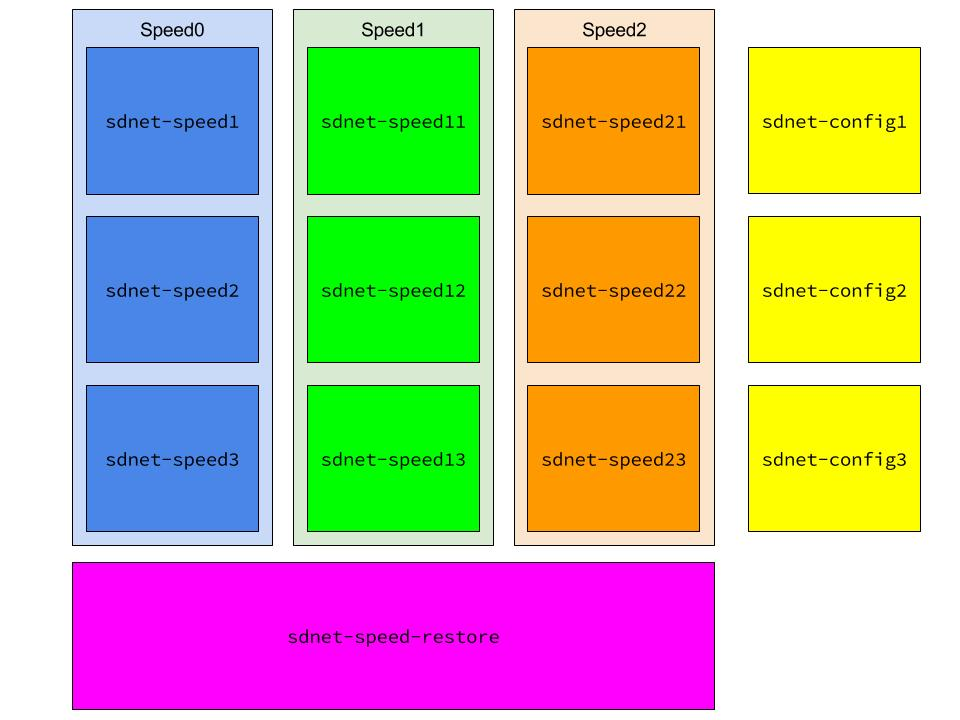
\includegraphics{production_cluster_schema.jpg}

I 3 config server sono i seguenti:
\begin{quote}

\begin{tabulary}{\linewidth}{|L|L|L|L|L|L|}
\hline
\textsf{\relax 
\textbf{Nodo}
} & \textsf{\relax 
\textbf{Host}
} & \textsf{\relax 
\textbf{\#CPU}
} & \textsf{\relax 
\textbf{RAM}
} & \textsf{\relax 
\textbf{Rete}
} & \textsf{\relax 
\textbf{Storage}
}\\
\hline
sdnet-config1
 & 
sdnet-config1.sdp.csi.it
 & 
1
 & 
4 GB
 & 
1 GB dati/1 GB backup
 & 
20 GB SO + 30 GB Dati
\\
\hline
sdnet-config2
 & 
sdnet-config2.sdp.csi.it
 & 
1
 & 
4 GB
 & 
1 GB dati/1 GB backup
 & 
20 GB SO + 30 GB Dati
\\
\hline
sdnet-config3
 & 
sdnet-config3.sdp.csi.it
 & 
1
 & 
4 GB
 & 
1 GB dati/1 GB backup
 & 
20 GB SO + 30 GB Dati
\\
\hline\end{tabulary}

\end{quote}

Le 3 shard sono così suddivise:
\begin{description}
\item[{speed0}] \leavevmode
\begin{tabulary}{\linewidth}{|L|L|L|L|L|L|}
\hline
\textsf{\relax 
\textbf{Nodo}
} & \textsf{\relax 
\textbf{Host}
} & \textsf{\relax 
\textbf{\#CPU}
} & \textsf{\relax 
\textbf{RAM}
} & \textsf{\relax 
\textbf{Rete}
} & \textsf{\relax 
\textbf{Storage}
}\\
\hline
sdnet-speed1
 & 
sdnet-speed1.sdp.csi.it
 & 
1
 & 
4 GB
 & 
1 GB dati/1 GB backup
 & 
20 GB SO + 110 GB Dati
\\
\hline
sdnet-speed2
 & 
sdnet-speed2.sdp.csi.it
 & 
1
 & 
4 GB
 & 
1 GB dati/1 GB backup
 & 
20 GB SO + 110 GB Dati
\\
\hline
sdnet-speed3
 & 
sdnet-speed3.sdp.csi.it
 & 
1
 & 
4 GB
 & 
1 GB dati/1 GB backup
 & 
20 GB SO + 110 GB Dati
\\
\hline\end{tabulary}


\item[{speed1}] \leavevmode
\begin{tabulary}{\linewidth}{|L|L|L|L|L|L|}
\hline
\textsf{\relax 
\textbf{Nodo}
} & \textsf{\relax 
\textbf{Host}
} & \textsf{\relax 
\textbf{\#CPU}
} & \textsf{\relax 
\textbf{RAM}
} & \textsf{\relax 
\textbf{Rete}
} & \textsf{\relax 
\textbf{Storage}
}\\
\hline
sdnet-speed11
 & 
sdnet-speed11.sdp.csi.it
 & 
1
 & 
4 GB
 & 
1 GB dati/1 GB backup
 & 
20 GB SO + 110 GB Dati
\\
\hline
sdnet-speed12
 & 
sdnet-speed12.sdp.csi.it
 & 
1
 & 
4 GB
 & 
1 GB dati/1 GB backup
 & 
20 GB SO + 110 GB Dati
\\
\hline
sdnet-speed13
 & 
sdnet-speed13.sdp.csi.it
 & 
1
 & 
4 GB
 & 
1 GB dati/1 GB backup
 & 
20 GB SO + 110 GB Dati
\\
\hline\end{tabulary}


\item[{speed2}] \leavevmode
\begin{tabulary}{\linewidth}{|L|L|L|L|L|L|}
\hline
\textsf{\relax 
\textbf{Nodo}
} & \textsf{\relax 
\textbf{Host}
} & \textsf{\relax 
\textbf{\#CPU}
} & \textsf{\relax 
\textbf{RAM}
} & \textsf{\relax 
\textbf{Rete}
} & \textsf{\relax 
\textbf{Storage}
}\\
\hline
sdnet-speed21
 & 
sdnet-speed21.sdp.csi.it
 & 
1
 & 
4 GB
 & 
1 GB dati/1 GB backup
 & 
20 GB SO + 110 GB Dati
\\
\hline
sdnet-speed22
 & 
sdnet-speed22.sdp.csi.it
 & 
1
 & 
4 GB
 & 
1 GB dati/1 GB backup
 & 
20 GB SO + 110 GB Dati
\\
\hline
sdnet-speed23
 & 
sdnet-speed23.sdp.csi.it
 & 
1
 & 
4 GB
 & 
1 GB dati/1 GB backup
 & 
20 GB SO + 110 GB Dati
\\
\hline\end{tabulary}


\end{description}

I 3 nodi di \textbf{backup} sono tutti sullo stesso host \code{sdnet-speed-restore} in modo da avere
una singola macchina dalla quale gestire i backup delle 3 {\hyperref[cluster_architecture/architecture:shard]{\emph{\DUspan{}{Shard}}}}:
\begin{quote}

\begin{tabulary}{\linewidth}{|L|L|L|L|L|L|}
\hline
\textsf{\relax 
\textbf{Nodo}
} & \textsf{\relax 
\textbf{Host}
} & \textsf{\relax 
\textbf{\#CPU}
} & \textsf{\relax 
\textbf{RAM}
} & \textsf{\relax 
\textbf{Rete}
} & \textsf{\relax 
\textbf{Storage}
}\\
\hline
sdnet-speed-restore
 & 
sdnet-speed-restore.sdp.csi.it
 &  &  &  & \\
\hline\end{tabulary}

\end{quote}


\chapter{Aggiunta di un nodo ad un replica set}
\label{cluster_architecture/add_replica:aggiunta-di-un-nodo-ad-un-replica-set}\label{cluster_architecture/add_replica::doc}\label{cluster_architecture/add_replica:add-replica}
Questo capitolo parla delle operazioni da effettuare per aggiungere un nodo ad un
{\hyperref[cluster_architecture/architecture:replica-set]{\emph{\DUspan{}{Replica set}}}} già esistente, è un'operazione che può essere eseguita ``a caldo'' senza
necessità di dare disservizio.

Per comodità il nuovo nodo verrà chiamato \code{sdnet-speed4.sdp.csi.it} e sarà aggiunto al
{\hyperref[cluster_architecture/architecture:replica-set]{\emph{\DUspan{}{Replica set}}}} \code{speed0}.
Nel caso in cui si voglia aggiungere un nodo con un host diverso, o nel caso in cui si voglia
aggiungere il nodo ad un differente {\hyperref[cluster_architecture/architecture:replica-set]{\emph{\DUspan{}{Replica set}}}} sarà necessario utilizzare i nomi corretti.


\section{Downlaod dei file necessari}
\label{cluster_architecture/add_replica:downlaod-dei-file-necessari}
Collegarsi tramite ssh al nuovo nodo:

\begin{Verbatim}[commandchars=\\\{\}]
\PYGZdl{} ssh sdnet\PYGZhy{}speed4.sdp.csi.it
\end{Verbatim}

Creare la cartella necessaria ad ospitare i file:

\begin{Verbatim}[commandchars=\\\{\}]
\PYGZdl{} mkdir \PYGZhy{}p /data/mongodb/conf/
\PYGZdl{} mkdir \PYGZhy{}p /data/mongodb/data/mongod\PYGZhy{}wiredTiger
...
\end{Verbatim}

Scaricare da un nodo già configurato del {\hyperref[cluster_architecture/architecture:replica-set]{\emph{\DUspan{}{Replica set}}}} i seguenti file: \code{mongod} (script
di avvio), \code{mongod.conf}, \code{keyfile}:

\begin{Verbatim}[commandchars=\\\{\}]
\PYGZdl{} sudo scp sdnet\PYGZhy{}speed1.sdp.csi.it:/etc/init.d/mongod /etc/init.d/mongod
\PYGZdl{} sudo scp sdnet\PYGZhy{}speed1.sdp.csi.it:/data/mongodb/conf/mongod.conf \PYGZbs{}
  /data/mongodb/conf/mongod.conf
...
\end{Verbatim}


\section{Restore dei dati}
\label{cluster_architecture/add_replica:restore-dei-dati}
\emph{Nel caso in cui si sta inizilizzando un nuovo :ref:{}`cluster{}` da 0 questo paragrafo si può
saltare.}

Per popolare il nuovo nodo con i dati esistono 2 possibilità:
\begin{itemize}
\item {} 
aggiungerlo al {\hyperref[cluster_architecture/architecture:replica-set]{\emph{\DUspan{}{Replica set}}}} ed aspettare che venga eseguita la sincronizzazione da 0

\item {} 
ripristinare i dati presi da un altro nodo

\end{itemize}

Vista la velocità e visto l'utilizzo di un nodo del {\hyperref[cluster_architecture/architecture:replica-set]{\emph{\DUspan{}{Replica set}}}} utilizzato esclusivamente
per il backup si è deciso di utilizzare la seconda possibilità.

Scaricare la cartella dei dati prendendola dal nodo di backup (\code{sdnet-speed-restore}):

\begin{Verbatim}[commandchars=\\\{\}]
\PYGZdl{} sudo scp \PYGZhy{}r sdnet\PYGZhy{}speed\PYGZhy{}restore.sdp.csi.it:/backup\PYGZus{}folder \PYGZbs{}
  /data/mongodb/data/mongod\PYGZhy{}wiredTiger
\end{Verbatim}

Lanciare l'istanza mongod:

\begin{Verbatim}[commandchars=\\\{\}]
\PYGZdl{} sudo /etc/init.d/mongod start
\end{Verbatim}


\section{Aggiunta al Replica Set}
\label{cluster_architecture/add_replica:aggiunta-al-replica-set}
Una volta lanciato il sever è necessario aggiungere al {\hyperref[cluster_architecture/architecture:replica-set]{\emph{\DUspan{}{Replica set}}}} il nuovo nodo appena
configurato, queste operazioni vanno eseguite sul {\hyperref[cluster_architecture/architecture:primary]{\emph{\DUspan{}{Primary}}}} del {\hyperref[cluster_architecture/architecture:replica-set]{\emph{\DUspan{}{Replica set}}}}.

Collegarsi al nodo \code{sdnet-speed1.sdp.csi.it} e verificare che sia {\hyperref[cluster_architecture/architecture:primary]{\emph{\DUspan{}{Primary}}}}:

\begin{Verbatim}[commandchars=\\\{\}]
\PYGZdl{} ssh sdnet\PYGZhy{}speed1.sdp.csi.it
\PYGZdl{} mongo \PYGZhy{}\PYGZhy{}port 27018
\PYGZgt{} use admin
\PYGZgt{} db.auth( \textbar{}db\PYGZus{}user\textbar{} , \textbar{}db\PYGZus{}password\textbar{} )
\PYGZgt{} db.isMaster()
\end{Verbatim}

Nel caso in cui sia {\hyperref[cluster_architecture/architecture:secondary]{\emph{\DUspan{}{Secondary}}}} provare con gli host \code{sdnet-speed2.sdp.csi.it} e
\code{sdnet-speed3.sdp.csi.it}

Una volta collegati al corretto {\hyperref[cluster_architecture/architecture:primary]{\emph{\DUspan{}{Primary}}}} aggiungere il nuovo nodo al {\hyperref[cluster_architecture/architecture:replica-set]{\emph{\DUspan{}{Replica set}}}}:

\begin{Verbatim}[commandchars=\\\{\}]
\PYGZgt{} rs.add(\PYGZdq{}sdnet\PYGZhy{}speed4.sdp.csi.it:27018\PYGZdq{})
\end{Verbatim}

Verificare che il nuovo nodo sia stato correttamente aggiunto:

\begin{Verbatim}[commandchars=\\\{\}]
\PYGZgt{} rs.conf()
\end{Verbatim}

Il \code{JSON} di output generato ha una chiave \code{members} in cui è presente la lista di tutti i
nodi del {\hyperref[cluster_architecture/architecture:replica-set]{\emph{\DUspan{}{Replica set}}}}, verificare che sia presente l'host del nuovo nodo appena aggiunto
(\code{sdnet-speed4.sdp.csi.it}).


\chapter{Inizializzazione di un Replica Set}
\label{cluster_architecture/init_replica_set:init-replica-set}\label{cluster_architecture/init_replica_set::doc}\label{cluster_architecture/init_replica_set:inizializzazione-di-un-replica-set}
Questa procedura servirà ogniqualvolta si vorrà aggiungere una nuova {\hyperref[cluster_architecture/architecture:shard]{\emph{\DUspan{}{Shard}}}} al
{\hyperref[cluster_architecture/architecture:cluster]{\emph{\DUspan{}{Cluster}}}} in quanto una {\hyperref[cluster_architecture/architecture:shard]{\emph{\DUspan{}{Shard}}}} deve essere necessariamente un {\hyperref[cluster_architecture/architecture:replica-set]{\emph{\DUspan{}{Replica set}}}}.

Per comodità il nuovo {\hyperref[cluster_architecture/architecture:replica-set]{\emph{\DUspan{}{Replica set}}}} verrà chiamato \code{speed3}, i relativo host che ne faranno
parte saranno \code{sdnet-speed31.sdp.csi.it}, \code{sdnet-speed32.sdp.csi.it},
\code{sdnet-speed33.sdp.csi.it}.
Nel caso in cui si voglia aggiungere una shard con un nome diverso, sarà necessario utilizzare i
nomi corretti.


\section{Downlaod dei file necessari}
\label{cluster_architecture/init_replica_set:downlaod-dei-file-necessari}
Collegarsi tramite ssh al nodo 1 del nuovo {\hyperref[cluster_architecture/architecture:replica-set]{\emph{\DUspan{}{Replica set}}}}:

\begin{Verbatim}[commandchars=\\\{\}]
\PYGZdl{} ssh sdnet\PYGZhy{}speed31.sdp.csi.it
\end{Verbatim}

Creare la cartella necessaria ad ospitare i file:

\begin{Verbatim}[commandchars=\\\{\}]
\PYGZdl{} mkdir \PYGZhy{}p /data/mongodb/conf/
\PYGZdl{} mkdir \PYGZhy{}p /data/mongodb/data/mongod\PYGZhy{}wiredTiger
...
\end{Verbatim}

Scaricare da un nodo già configurato del {\hyperref[cluster_architecture/architecture:replica-set]{\emph{\DUspan{}{Replica set}}}} i seguenti file: \code{mongod} (script
di avvio), \code{mongod.conf}, \code{keyfile}:

\begin{Verbatim}[commandchars=\\\{\}]
\PYGZdl{} sudo scp sdnet\PYGZhy{}speed1.sdp.csi.it:/etc/init.d/mongod /etc/init.d/mongod
\PYGZdl{} sudo scp sdnet\PYGZhy{}speed1.sdp.csi.it:/data/mongodb/conf/mongod.conf \PYGZbs{}
  /data/mongodb/conf/mongod.conf
...
\end{Verbatim}


\section{Cambio dei parametri di configurazione}
\label{cluster_architecture/init_replica_set:cambio-dei-parametri-di-configurazione}
Nel file di configurazione \code{mongod.conf} appena scaricato andare a modificare il valore della
chiave \code{replSet} mettendo il nome del nuovo {\hyperref[cluster_architecture/architecture:replica-set]{\emph{\DUspan{}{Replica set}}}}:

\begin{Verbatim}[commandchars=\\\{\}]
\PYG{n}{replSet}\PYG{o}{=}\PYG{n}{speed0}
\end{Verbatim}


\section{Inizializzazione del Replica Set}
\label{cluster_architecture/init_replica_set:inizializzazione-del-replica-set}
Lanciare l'istanza \code{mongod}:

\begin{Verbatim}[commandchars=\\\{\}]
\PYGZdl{} sudo /etc/init.d/mongod start
\end{Verbatim}

Collegarsi al \code{mongod} appena lanciato utilizzando la shell \code{mongo}:

\begin{Verbatim}[commandchars=\\\{\}]
\PYGZdl{} mongo \PYGZhy{}\PYGZhy{}port 27017
\end{Verbatim}

Inizializzare il {\hyperref[cluster_architecture/architecture:replica-set]{\emph{\DUspan{}{Replica set}}}}:

\begin{Verbatim}[commandchars=\\\{\}]
\PYGZgt{} rs.initiate()
\end{Verbatim}


\section{Aggiungere gli altri nodi}
\label{cluster_architecture/init_replica_set:aggiungere-gli-altri-nodi}
Per aggiungere gli altri nodi al {\hyperref[cluster_architecture/architecture:replica-set]{\emph{\DUspan{}{Replica set}}}} seguire la procedura illustrata nel capitolo
{\hyperref[cluster_architecture/add_replica::doc]{\emph{\emph{Aggiunta di un nodo ad un replica set}}}}


\chapter{Aggiunta di una shard al cluster}
\label{cluster_architecture/add_shard:add-shard}\label{cluster_architecture/add_shard::doc}\label{cluster_architecture/add_shard:aggiunta-di-una-shard-al-cluster}
Una {\hyperref[cluster_architecture/architecture:shard]{\emph{\DUspan{}{Shard}}}} deve essere obbligatoriamente un {\hyperref[cluster_architecture/architecture:replica-set]{\emph{\DUspan{}{Replica set}}}}, nel caso in cui non sia già
stato configurato un nuovo {\hyperref[cluster_architecture/architecture:replica-set]{\emph{\DUspan{}{Replica set}}}}, è necessario procedere alla sua inizializzazione
seguendo quanto spiegato nel capitolo {\hyperref[cluster_architecture/init_replica_set::doc]{\emph{\emph{Inizializzazione di un Replica Set}}}}.

L' operazione di aggiunta di una nuova {\hyperref[cluster_architecture/architecture:shard]{\emph{\DUspan{}{Shard}}}} può essere eseguita ``a caldo'' senza necessità
di dare disservizio, considerare comunque che sarà poi necessario che il \code{balancer} migri i
\code{chunk} di dati e potrebbe causare un degrado del servizio.

Per comodità la {\hyperref[cluster_architecture/architecture:shard]{\emph{\DUspan{}{Shard}}}} aggiunta verrà chiamata \code{speed3}, il relativo host scelto per
fare l'aggiunta al {\hyperref[cluster_architecture/architecture:cluster]{\emph{\DUspan{}{Cluster}}}} sarà \code{speed3/sdnet-speed31.sdp.csi.it}.
Nel caso in cui si voglia aggiungere una {\hyperref[cluster_architecture/architecture:shard]{\emph{\DUspan{}{Shard}}}} con un nome diverso, sarà necessario
utilizzare i nomi corretti.


\section{Collegamento a mongos}
\label{cluster_architecture/add_shard:collegamento-a-mongos}
Collegarsi tramite ssh ad un nodo avente un {\hyperref[cluster_architecture/architecture:mongos]{\emph{\DUspan{}{Mongos}}}} in esecuzione:

\begin{Verbatim}[commandchars=\\\{\}]
\PYGZdl{} ssh sdnet\PYGZhy{}speed1.sdp.csi.it
\end{Verbatim}

Collegarsi al {\hyperref[cluster_architecture/architecture:mongos]{\emph{\DUspan{}{Mongos}}}} utilizzando la shell \code{mongo} e autenticarsi:

\begin{Verbatim}[commandchars=\\\{\}]
\PYGZdl{} mongo \PYGZhy{}\PYGZhy{}port 27019
\PYGZgt{} use admin
\PYGZgt{} db.auth( \textbar{}db\PYGZus{}user\textbar{} , \textbar{}db\PYGZus{}password\textbar{} )
\end{Verbatim}


\section{Aggiunta della shard}
\label{cluster_architecture/add_shard:aggiunta-della-shard}
Aggiungere la {\hyperref[cluster_architecture/architecture:shard]{\emph{\DUspan{}{Shard}}}} al {\hyperref[cluster_architecture/architecture:cluster]{\emph{\DUspan{}{Cluster}}}}, specificando prima il nome del {\hyperref[cluster_architecture/architecture:replica-set]{\emph{\DUspan{}{Replica set}}}}
seguito dall' host di uno dei membri:

\begin{Verbatim}[commandchars=\\\{\}]
\PYGZgt{} sh.addShard( \PYGZdq{}speed3/sdnet\PYGZhy{}speed31.sdp.csi.it\PYGZdq{} )
\end{Verbatim}


\chapter{Inizializzazione del cluster}
\label{cluster_architecture/init_cluster:inizializzazione-del-cluster}\label{cluster_architecture/init_cluster:init-cluster}\label{cluster_architecture/init_cluster::doc}
todo



\renewcommand{\indexname}{Index}
\printindex
\end{document}
